\documentclass[journal]{./sty/IEEEtran}

\usepackage{graphicx}

% *** CITATION PACKAGES ***
\usepackage{cite}
% cite.sty was written by Donald Arseneau
% V1.6 and later of IEEEtran pre-defines the format of the cite.sty package
% \cite{} output to follow that of IEEE. Loading the cite package will
% result in citation numbers being automatically sorted and properly
% "compressed/ranged". e.g., [1], [9], [2], [7], [5], [6] without using
% cite.sty will become [1], [2], [5]--[7], [9] using cite.sty. cite.sty's
% \cite will automatically add leading space, if needed. Use cite.sty's
% noadjust option (cite.sty V3.8 and later) if you want to turn this off.
% cite.sty is already installed on most LaTeX systems. Be sure and use
% version 4.0 (2003-05-27) and later if using hyperref.sty. cite.sty does
% not currently provide for hyperlinked citations.
% The latest version can be obtained at:
% http://www.ctan.org/tex-archive/macros/latex/contrib/cite/
% The documentation is contained in the cite.sty file itself.


% *** MATH PACKAGES ***
%
\usepackage[cmex10]{amsmath}
% A popular package from the American Mathematical Society that provides
% many useful and powerful commands for dealing with mathematics. If using
% it, be sure to load this package with the cmex10 option to ensure that
% only type 1 fonts will utilized at all point sizes. Without this option,
% it is possible that some math symbols, particularly those within
% footnotes, will be rendered in bitmap form which will result in a
% document that can not be IEEE Xplore compliant!
%
% Also, note that the amsmath package sets \interdisplaylinepenalty to 10000
% thus preventing page breaks from occurring within multiline equations. Use:
% \interdisplaylinepenalty=2500
% after loading amsmath to restore such page breaks as IEEEtran.cls normally
% does. amsmath.sty is already installed on most LaTeX systems. The latest
% version and documentation can be obtained at:
% http://www.ctan.org/tex-archive/macros/latex/required/amslatex/math/


\usepackage{url}


% correct bad hyphenation here
\hyphenation{net-works SpiNNaker depending}

\begin{document}
%
% paper title
% can use linebreaks \\ within to get better formatting as desired
\title{Effects Of Real-time Synaptic Plasticity Using Spiking Neural Network Architecture
}


\author{Matthew Frazier ~
        Nishant Shukla ~
        Worthy Martin* }

% The paper headers
%\markboth{Journal of Neuroscience Methods,~Vol.~x, No.~y, May~2014}%
%{Shell \MakeLowercase{\textit{et al.}}: Synaptogenesis on the SpiNNaker}
% The only time the second header will appear is for the odd numbered pages
% after the title page when using the twoside option.

\markboth{Synaptogenesis on the SpiNNaker, May~2014}%
{Shell \MakeLowercase{\textit{et al.}}: Synaptogenesis on the SpiNNaker}


% make the title area
\maketitle

\begin{abstract}
Artificial Neural Networks is a promising approach to study human brain computation in hopes of achieving similar learning by artificial agents.
Recent architecture design of a low-power supercomputer by the University of Manchester, the SpiNNaker,
has made it easier to design highly parallel brain-inspired algorithms.
We used the SpiNNaker machine to implement a neural network capable of rewiring its connection 
in real-time while trying to minimize information loss and maximize the decrease in statistical dependence.
We believe this is the first use of synaptogenesis on a spiking neural network architecture, 
laying the framework for future efficient brain-like neural networks.
Additionally, we explored scalability issues and unintended pitfalls with this approach.

\end{abstract}

\begin{IEEEkeywords}
Neural Networks, Synaptogenesis, SpiNNaker
\end{IEEEkeywords}


%% TODO: Nishant
\section{Introduction}
\IEEEPARstart{A}{rtificial} neural networks often require vast amounts of computation memory and space \cite{CorrMatr:Levy}.
Some of the most effective algorithms such as back propagation do not scale well for a network consisting of a billion or more neurons \cite{backprop:Qun}.
Furthermore, most neural network models do not fully utilize the machine on which they run. 
The ones that do fully utilize their machine are typically implemented on Graphical Processing Units (GPUs) which disproportionately drain energy.

Finding a solution to revive neural networks to the same computational caliber 
as other paradigms, such as Support Vector Machines (SVM), would better adhere to biologically based design.
Studying biologically inspired structures as opposed to statistically based ones allows us to grasp a better understanding of the human brain.
By designing a neural network experiment on a new kind of computer architecture, 
this paper aims to demonstrate the high performing nature of neural networks.

Recently, deep feedforward neural networks have risen in popularity \cite{DNN:Siniscalchi}. 
Multiple deep-learning approaches have proven to be practical.
However, a major issue with deep-learning is the computation time for large networks.
Deep-learning does not scale well due to the innate use of back-propagation in the algorithm.

Our approach to neural network learning is through an unsupervised model on a spiking neural network architecture.
By utilizing almost every core of the 72-core energy-efficient embedded system, 
we are capable of reproducing complex neural network patterns in less than half the energy-cost. 
The network creates and removes synapses in real-time, so not only are weights learned and adjusted simultaneously, 
but so are the actual connections between the neurons.
We demonstrate that introducing synaptic modification on a neural network leads to a biologically accurate model
that outperforms previous methods in both performance and energy costs \cite{MPI:Plana}.


\section{Background}
\IEEEPARstart{T}{he} subfield of AI known as neural network computation has recently received a large and growing amount of attention. 
Put simply; neural networks (NN) are computational models inspired by biological brains that are capable of machine learning. 
A NN usually consists of interconnected "neurons" (in quotation marks for they are artificially simulated to varying degrees of biological accuracy -- but that topic is outside the scope of this paper) which compute from their inputs and produce various outputs, depending on the model. 

This paper focuses on types of spiking neural network (SNN) models, in which the neuronal communication (and therefore, the computation of the system as a whole) is achieved via message spikes, or action potentials, from one neuron that is synapsed onto another. 
In this introduction, we first describe how a SNN is a good computational representation of the brain. 
We then describe various different spike-dependent spike-time learning methods used on a SNN, followed by an exploration of various types of SNN. 
We discuss why the neuromimetic hardware we use is a good platform for experimentation with SNN \cite{HierarchMPA:Galluppi}, and then describe our approach to the problem of simulating synaptogenesis on such a device and propose a solution. 
Our design and implementation sections explore this solution in detail, 
and our results section describe the outcome of our experiment.
Furthermore, we discuss future work that remains to be conducted, including interesting implications such as computability beyond Von Neuman architecture and Turing machines.

\subsection{The Brain And Other Spiking Neural Networks}
The brain is a spiking neural network. 
That is to say; biological neurons pass information around the brain via action potentials which travel from a neurons' soma (cell body) down the axon and generate synaptic events which are received by the dendrites of all other connected neurons.
Figure~\ref{fig:neuron} diagrams the relevant biological prerequisites.

\begin{figure}
\centering
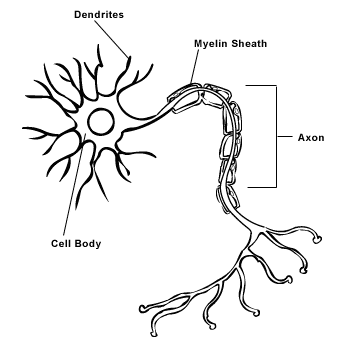
\includegraphics[scale=0.6]{imgs/neuron.png}
\caption{Visual representation of a biological neuron identifying the cell body, dendrites, axon, and myelin sheath. 
Source: \cite{img:N} \label{fig:neuron}}
\end{figure}


The process has been simplified greatly as neurobiology is not the focus of this paper, nor are the biological processes yet completely understood. 
What is important are the overarching properties exhibited by brains. 
Namely; that brains are fast, power-efficient, and capable of obtaining, representing, and integrating complex multi-dimensional information sets into useful knowledge (from unreliable sensory inputs, at that). 
Moreover, the property of being able to fairly reliably solve highly complex problems is something we want computers to have. 
Progress is however being made towards the goal of making machines more like minds; indeed, the bus in a computers' hardware may operate at tens of MHz, while an axon may carry only tens to hundreds of action potentials per second, about five orders of magnitude slower than a machine \cite{NSE:Furber}. 
The power efficiency of the brain is still far ahead of even the best neuromimetic hardware but the gap is closing quickly, considering that biological evolution had several hundred million years of a head start. 

One very important property of the brain that has received little attention by computer scientists, which is also believed to be quintessential in mankind's ability to adapt to and solve new and ever-more difficult problems, is neural plasticity involving the dynamic creation or removal of synapses.
It would be erroneous to say that no degree of plasticity has been implemented in any type of SNN, but to the best of our knowledge there is yet no model which allows networks to add or remove synapses at runtime. 
Given that we do not yet fully understand the mechanisms governing neural plasticity in our own heads, it suffices to say that there is yet much work to be done in this field of computational neuroscience in which artificial neural networks dynamically alter their own topology \cite{ENNtAT:Stanley}.

\subsection{Overview of Spike-time coding and learning methods}
Before discussing different types of artificial spiking neural networks, 
it is necessary to describe various spike-time coding and learning methods 
that are relevant to understanding how the different types of spiking neural networks function.

Firstly, the distinction between rate- and rank-order coding must be addressed. 
Rate order coding is, as it sounds, a way to describe neural responses to stimulus 
in terms of firing rate, paying attention to the timing between spikes of a single input. 
Rank order, on the other hand, focuses on the relative timing of spikes from all inputs \cite{RankPolychron:Galluppi}. 
Rate order has a number of drawbacks, though the primary one is its inability to transmit 
and process information in a short period of time; with \(n\) neurons being able 
to transmit over the course of 10 ms only $log_2(n C 1)$ bits of information \cite{RO:Thorpe}.
Rank order, under the same constraints, is capable of achieving $log_2(n!)$ bits of information \cite{deSNN:Kasabov}.

As detailed in \cite{RO:Thorpe}, rate order can be considered an $analog-to-frequency$ converter, while rank order would be an $analog-to-delay$ converter, as the time an integrate-and-fire neuron takes to reach threshold is dependent upon input strength. 
During an initial learning phase, in which a new output neuron $i$ is created for each $N$-dimensional training input pattern, connection weights $w_j,i (j = 1,2,...,N)$ are calculated based on the rank order learning rule:

\begin{equation}
w_j,i(t) = {\alpha}\cdot{mod^{order(j,i)}} 
\end{equation} 
where $w_j,i$ is the connection weight between post-synaptic neuron $i$ and pre-synaptic neuron $j$, $\alpha$ is a learning parameter, $mod$ is a modulation factor (determining the importance of the order of the first spikes), with $order(j,i)$ representing the order of spikes arriving at neuron $i$ from all synapses to the neuron $i$ (has value $0$ for the first spike to neuron $i$, increases incrementally for each subsequent spike from other pre-synaptic neurons) \cite{deSNN:Kasabov}.
Some models using rank order coding will also merge output neurons with similar weight vectors based on the Euclidean distance between them, thus reducing the number of redundant neurons that must be simulated.
In short, rank order (RO) coding is assumed to be a better basis for model construction as it allows networks to process more information in a shorter amount of time with fewer redundant neurons \cite{RO:Thorpe}.
One of the only downsides to rank order over rate order is a slightly increased computational overhead.

Moving on to learning methods, spike time dependent plasticity (STDP) implements plasticity 
through the use of long-term potentiation (LTP) and depression (LTD) \cite{FBBPSTDP:Davies, FBSTDP:Davies, STDPonset:Humble}.
Put simply, the connection weight between two neurons increases 
if the pre-synaptic neuron spikes before the post-synaptic neuron, 
and the weight decreases in the reverse case.  
Spike driven synaptic plasticity (SDSP) is a semi-supervised variant of STDP 
in which a threshold $Vmth$ is given to the post-synaptic neurons' membrane potential \cite{deSNN:Kasabov}.
If the membrane potential is above $Vmth$ when an input spike arrives, potentiation occurs. 
Otherwise, the synapse experiences depression.
These two cases are typically either shortly before or shortly after a post-synaptic 
spike is emitted, respectively. 

STDP is the most commonly discussed paradigm for learning in neural networks. Its benefits include its unsupervised nature, and, significantly, the ability for the LTP and LTD weight modifications to be calculated by the post-synaptic neuron upon receipt of a spike. This allows the updates to be performed at a single point in the simulation: at the spike arrival event, which can further increase the efficiency of a simulation \cite{FBBPSTDP:Davies,FBSTDP:Davies}.

We will later describe a new learning method referred to as synaptogenetic spike time dependent plasticity (SSTDP), utilizing STDP and governed by biologically inspired synaptogenetic formulas taken from \cite{SynGen:Levy}, and influenced by Information Theory from Shannon.

\subsection{Types of Spiking Neural Networks}
\begin{itemize}
\item[(a)] {\bf A spiking neural network (SNN)} is the most basic form, 
in which synaptic weights are static and neurons communicate via message spikes.
While they have some drawbacks, an SNN is still a fairly powerful biologically-inspired model.
\item[(b)] {\bf An evolving spiking neural network (eSNN)} evolves its functionality and 
structure based on incoming information using the RO rule, 
but only during a learning phase \cite{deSNN:Kasabov}.
Once a neurons' weight has been set, however, this model does not allow 
for any further tuning of synaptic weights to reflect on other incoming spikes at the same synapse. 
That is to say; these synapses can capture some long-term memory during the learning phase, 
but have little ability to capture any short term memory, which is detrimental to the computational 
capabilities of the network as a whole \cite{deSNN:Kasabov}.
\item[(c)] {\bf A dynamically evolving spiking neural network (deSNN)} represents an improvement 
over eSNN in that it implements not only RO learning during an initial learning phase, 
but also a dynamic synaptic plasticity mechanism so that it will continue to learn and 
improve performance during a recall phase; the deSNN proposed in \cite{deSNN:Kasabov} 
uses the SDSP mechanism. 
This fixes the primary shortcoming of the eSNN model; 
allowing for short term memory to be stored easily, 
and to be potentiated as long as it remains useful\cite{deSNN:Kasabov}. 
\end{itemize}

\subsection{SpiNNaker}
The Spiking Neural Network Architecture (SpiNNaker) board is a neuromimetic hardware 
system designed by the University of Manchester with the eventual intent of simulating 
the human brain. Each SpiNNaker processing node is a multicore system-on-chip (SoC) 
with 1GB SDRAM, containing 18 ARM968 processor cores, connected in a toroidal triangular 
mesh with passed messages being managed by an on-chip router for an asynchronous 
packet-switched network-on-chip (NoC) \cite{GALS:Plana}.
It is the brainchild of Steve Furber, and has a number of properties that make it 
useful for neural computation:
\begin{itemize}
\item[(a)]{\bf Fast:}
The SpiNNaker system has a bisection bandwidth of over 5 billion 
packets/s \cite{ArchOverV:Furber}. It is, by design, meant to model spiking neural networks 
in real time. However, it can be said to outperform biology in terms of raw speed of neural activity \cite{RTS:Davies}, 
and must be slowed down to run real-time simulations \cite{ArchOverV:Furber, Fast:Rast}.
\item[(b)]{\bf Power efficient:} A simulation run on the SpiNNaker system has been documented taking 100 nJ per neuron per 
millisecond and 43 nJ per postsynaptic potential, a smaller power consumption than any other 
recorded digital simulation \cite{Efficient:Sharp}.
\item[(c)] {\bf Massively parallelized:} The brain is a massively parallel system populated with many low-performance asynchronous components 
known as neurons \cite{BioMPA:Furber}. It follows that a digital system meant to effectively and 
efficiently emulate neural activity would also be massively parallelized \cite{Interconnection:Navaridas}, though each ARM core is 
substantially more complex than a single neuron, and can efficiently model many neurons in 
real time \cite{ArchOverV:Furber}. Each NoC is extended seamlessly to surrounding chips, 
creating a power-efficient system-wide interprocessor communication network \cite{GALS:Plana}.
\item[(d)]{\bf Globally asynchronous, locally synchronous (GALS)} In a GALS system, individual processing cores have their own clock signals, potentially 
with different frequencies, and require no interprocessor phase-alignment \cite{GALS:Plana}. 
Each SpiNNaker chip is its own GALS system, with an independently-clocked router managing 
intercore and interchip communications, leading to the SpiNNaker system as a whole also 
being a GALS system \cite{BioMPA:Furber}. 
Major benefits of a GALS approach include that it eliminates any top-level 
system constraints (i.e. it is decentralized), 
and any timing closure issues \cite{GALS:Plana}. 
It also offers increased flexibility regarding process variability \cite{BioMPA:Furber}.
\item[(e)]{\bf Fault Tolerant:} In any large-scale systems fault tolerance is a major concern, and is increases in importance 
with the number of fallible subsystems \cite{ArchOverV:Furber}.
Fault tolerance was paid a great deal of attention by the SpiNNaker development team, 
and listing all the built-in mechanisms at various levels of abstraction is outside the scope 
of this paper. 
To summarize, fault tolerance mechanisms exist at nearly every level of the system, 
including those related to processors, 
the interrupt controller, timers, and packet communications, 
allowing subsystems to generally fail gracefully without greatly affecting 
the performance of the system as a whole \cite{ArchOverV:Furber}.
\item[(f)]{\bf Scalable:} Due to the nature inherent to its GALS design, it is arbitrarily scalable. 
The only cost associated with scaling up the system is power consumption. 
The full million-core machine has an expected power budget of around 90 kW \cite{ArchOverV:Furber}.
\end{itemize}

To summarize, the SpiNNaker specifically disregards three significant axioms of conventional supercomputing (memory coherence, synchronization, determinism) in a way that makes it well-suited for a wide range of biological and non-biological applications \cite{ArchOverV:Furber}.

\subsection{Synaptic Plasticity}
A difficult problem in designing neural networks is configuring the initial parameters to optimize the network.
For example, defining how the neurons are connected together greatly affects the efficiency and performance in learning \cite{SynGen:Levy}.
Perceptrons are often designed as bipartite graphs, where every neuron in the pre-synaptic layer is connected to every neuron in the post-synaptic layer.
This brute-force approach to constructing a network topology may achieve satisfactory results if the weights converge to the optimal values within an acceptable time.
However, a bipartite graph scales exponentially to the number of nodes in each layer. 
In our solution, we let the neural network modify itself, providing a ``hands-off'' approach to designing a network.

Other than updating synaptic weights to achieve learning, we introduce two additional forms of synaptic plasticity. 
In our study, we allow new synapses to be formed (synaptogenesis), or existing synapses to be entirely disconnected. 
The three types of plasticity undergo the following principles \cite{SynGen:Levy, SynGen2:Levy}:

\begin{itemize}
\item[(a)] {\bf Synaptogenesis} - 
Unlike most networks, we allow ours to form new connections between neurons while learning occurs. 
The creation of a new synapse depends on whether the post-synaptic neuron is at an optimal activation. 
If not, the network considers forming a new synapse.
Additionally, synaptogenesis only occurs between neighboring neurons, ensuring a constraint on locality.
Synapses are formed by taking into account both receptivity and avidity \cite{SynGen:Levy, SynGen2:Levy}.

\vspace{0.3cm}

Avidity is the measure of ability for each neuron to participate in a new synaptic connection, defined as

\[
A_i(t)=\frac{a}{(a + \sum_j\sum_kW_{i_kj}(t))}
\]

\[
a = \left\{
\begin{array}{lr}
  1.0 * 10^{33} & \text{for unlimited avidity}\\
  1.0 & \text{for moderate avidity}\\
  1.0 * 10^{-3} & \text{for limiting avidity}
\end{array}
\right.
\]

The receptivity of new synaptic connections is inversely proportional to the running average of the neuron's activation.
We use the following equation for receptivity,

\[
R_j(t) = \frac{r_1}{r_1 + \bar{y}_j(t)^{r_2}}
\]

\[
\bar{y}(t) = 0.99 \bar{y}_j(t-1) + 0.01 Y_j(t)
\]

\[
\text{(\(r_1\) and \(r_2\) are experimental constants)}
\]

Finally, the probability of forming a new synapse between two neurons \(i\) and \(j\) depends on both avidity and receptivity. 

\[
\text{Prob}(\text{of new synapse } ij ) \propto A_i(t) * R_j(t)
\]

\item[(b)] {\bf Weight Modification} - 
Similar to most unsupervised weight modification rules, we use a deterministic process depending on the pre- and post-synaptic activities.
This type of weight adjustment is based off the Hebbian rule, where links between nodes that fire together strengthens.
Specifically, weights are adjusted using the following formula,

\[
\triangle w(t+1) \propto f(\text{post}_j(t))*g(\text{pre}_j(t), w_{ij}(t))
\]

\item[(c)] {\bf Synapse Removal} -
Lastly, we allow our network to undergo synaptic removal, a stochastic process where the probability of removal becomes non-zero if excitatory synapses fall bellow a specified threshold.
Given some constant \(\delta > 0\), probability of synaptic removal is defined as

\[
\text{Prob}(\text{removal } ij) = \left\{
     \begin{array}{lr}
       0 & \text{if } w_{ij}(t) + \triangle w_{ij}(t+1) > \delta\\
       >0 & \text{otherwise}
     \end{array}
   \right.
\]

\end{itemize}

Synaptic connections are slowly modified through additions or removals until optimal output firing levels are obtained. 

Levy asserts that  ``information theory has gained popularity in recent years as a tool for understanding brain recordings.''


\section{Design}
\IEEEPARstart{N}{eural} networks consist of biologically inspired relationships between individual nodes (neurons). Learning in such a network occurs by intelligently adjusting weights on the links between the nodes. We define the relationship between nodes into the following three categories:

\begin{itemize}
\item[(a)] {\bf Static} - where the network topology is fixed, and can only change by manually adjusting the relationship between nodes. Most neural networks fall into this category because regardless of the number of nodes \(n\), only one fixed relationship forms between them:

\[
\text{NumberOfTopologies}(n) = 1
\]


\item[(b)] {\bf Semi-Dynamic} - in which the network is not static, and there is some freedom for nodes to rewire with other nodes in real time. The complexity grows exponentially. Each node has non-zero probability to be rewired with a constant \(c\) number of other nodes. Given \(n\) such nodes, the number of possible topologies can be up to

\[
\text{NumberOfTopologies}(n) = c^n
\]


\item[(c)] {\bf Dynamic} - where each node has non-zero probability to be wired with any other neuron in the entire network. Given \(n\) nodes, the number of possible topologies becomes

\[
\text{NumberOfTopologies}(n) = n^{n-1}
\]


\end{itemize}

A biological neural network such as the human brain does not follow the static network topology. 
Connections between neurons in the brain are regularly formed and removed over time \cite{SynGen:Levy, StatDepRed:Levy}. 
Moreover, such a neural network is not fully dynamic either, since locality is a physical constraint. 
For example, a neuron on the far end of the left hemisphere of a brain might never directly connect with a neuron on the right hemisphere.

We designed a programming framework on SpiNNaker's interface to enable a semi-dynamic network topology.
Each neuron has the flexibility to rewire with none, all, or some of the fixed number of other neurons, following our synaptic plasticity rules.
To test performance, the network analyzed the MNIST database of handwritten digits. We compared information loss (see appendix A) from a network following our synaptic plasticity model, to that without synaptogensis and synapse removal.

% 5 neurons can have 14 polygroups, and 6 can have twice as much. 
% Ergo, human brain has a bunch.
% Which may be a cause of intelligence? Our implementation will mimic this.

In order to implement a spiking neural network, we choose an existing neural model.
There exists multiple neural models for implementing a spiking neural network. 
Some of the most popular models are briefly covered below.
 
\begin{itemize}
\item[(a)] {\bf Integrate-and-fire (IF)} 
 is one such model which increments the voltage while a current is present,
and finally resets the voltage once a threshold $V_{th}$ is reached. 
Every voltage reset produces a spike for that neuron.
While computationally efficient, the IF model does not exhibit properties of the cortical spiking neurons.
\item[(b)] {\bf Leaky integrate-and-fire (LIF)} 
 models are a biologically revised version of the previous model.
This model allows for ``forgetting'' isolated input currents.
However, it also is insufficient for modeling cortical spiking neurons.
\item[(c)] {\bf Izhikevich} 
 model is an adaptation of the Integrate-and-fire model that uses a quadratic non-linearity when adjusting the voltage.
This model is known for its applicability to large-scale simulations of cortical neural networks \cite{Spikes:Izhi, Polychron:Izhi}.
\end{itemize}

We use the Izhikevich model since it our best candidate for a biologically inspired neuron
that is simple enough to implement on a new computer architecture. 
By running an ensemble of neurons on the SpiNNaker, 
we wish to see both a more energy and time efficient approach for emulating neural networks.
In direct comparison to Izhikevich's paper on polychronization, 
we present a spiking neural network on the SpiNNaker 
that can also exhibit reproducible time-locked but not synchronous firing patterns.
This time-lock pattern is referred to as polychronization \cite{Polychron:Izhi}.

These polygroups are possible due to introducing delays in the network.
The SpiNNaker machine produces natural delays as packets are sent to and from chips.
We take advantages of the delays to discover these polygroups.
A network of five neurons with embedded delays can produce fourteen polygroups.
Generally, the number of polygroups is exponentially greater than the number of neurons in a network, 
as long as the delays are properly synchronized. 
The human brain consists of over $10^{11}$ neurons, which have the capability of producing even more polygroups.
With our implementation, we aim to uncover the polygroups from the machine's innate delays.

% TODO: Nishant, Talk about how SpiNNaker float stuff is implemented
% and parallel architecture design, STDP implementation
% and spnet here
\section{Implementation}
\IEEEPARstart{B}{y} taking advantage of the multiple independent cores on the SpiNNaker, we were able to emulate efficient real-time synaptogenesis. The neural network consisted of 39 excitatory input neurons, 9 inhibitory input neurons, and 16 excitatory output neurons. 

\subsection{Input Spikes}
The SpiNNaker neural network was given a set of letters as input. 
Each letter was represented by a 48-dimensional binary vector of $1s$ or $0s$. Figures~\ref{fig:U} and~\ref{fig:V} are examples of letters with fairly similar input vectors, for illustration.

\begin{figure}
\centering
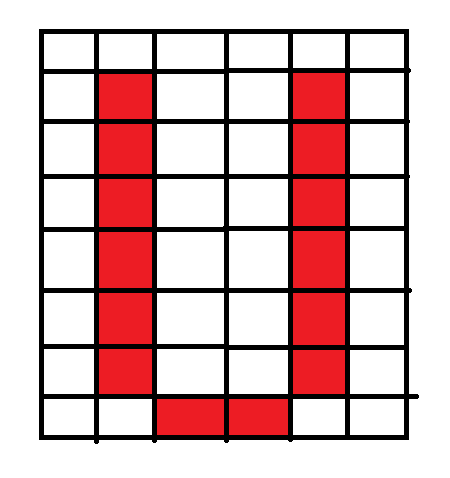
\includegraphics[scale=0.3]{imgs/U.png}
\caption{The letter U.\label{fig:U}}
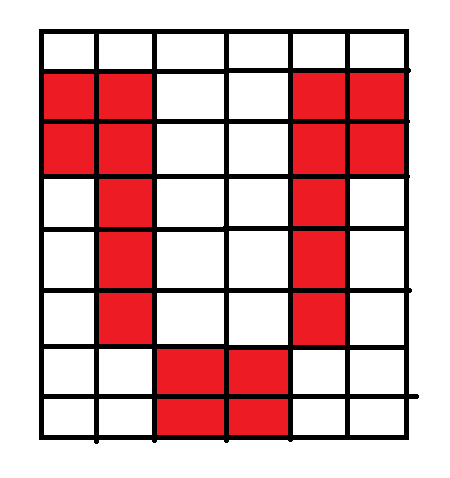
\includegraphics[scale=0.3]{imgs/V.png}
\caption{The letter V.\label{fig:V}}
\end{figure}

Intuitively, a $1$ represents a colored pixel, and a $0$ represents a blank pixel in a visual $8$ x $6$ image representation of the letter. 
Each coordinate of the 48-dimensional input spikes its corresponding input neuron. Figure~\ref{fig:A} shows a letter with its input vector.

\begin{figure}
\centering
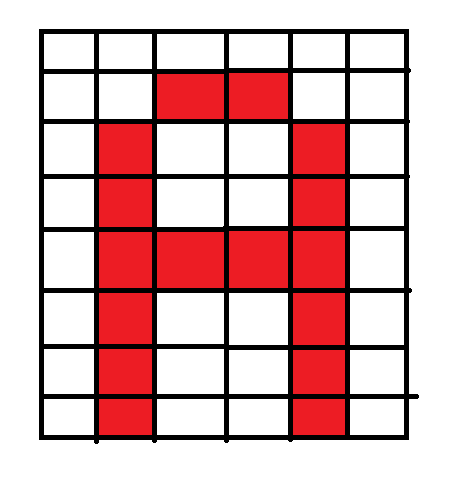
\includegraphics[scale=0.3]{imgs/A.png}
\caption{000000001100010010010010011110010010010010010010\label{fig:A}}
\end{figure}
o
The letters were randomly generated by a Python script which sends a spike to the SpiNNaker machine serially. Three chips receive the input generated by the Python script, and feed their generated spikes to the fourth as an output chip, illustrated in figure~\ref{spinnIO}.

\begin{figure}
\centering
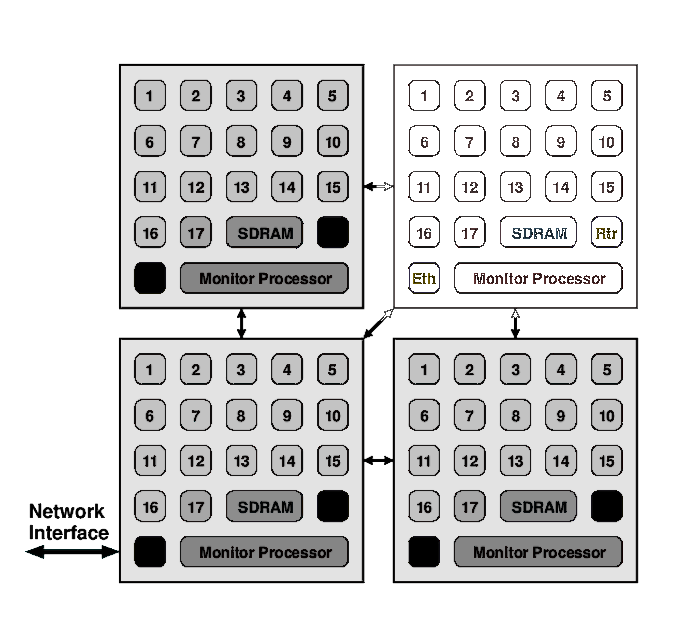
\includegraphics[scale=0.3]{imgs/SpiNN4IO.png}
\caption{Illustration of three Input and one Output chips\label{spinnIO}}
\end{figure}


\subsection{Floating Point Arithmetic}
The SpiNNaker machine has no hardware support for floating point arithmetic \cite{ArchOverV:Furber}. 
However, the Izhikevich neural model adjusts voltage variables based off the following equations.

\begin{math}
\triangle v = 0.04 v^2 + 5 v  + 140 - u + I
\end{math}

\begin{math}
\triangle u = a(b v - u)
\end{math}

In order to alleviate the rounding errors from only using integer arithmetic on the SpiNNaker machine, 
we scale the equations up to remove all floating points values. 
Then we use integer division in the final step to obtain the actual result.
The rounding errors of implementing the Izhikevich model are typically minute if apparent at all, shown in the figures~\ref{fig:tonic} through~\ref{fig:excit1} and~\ref{fig:excit2} through~\ref{fig:accomod8}. This is discussed in greater detail in appendix B.

\begin{figure}
\centering
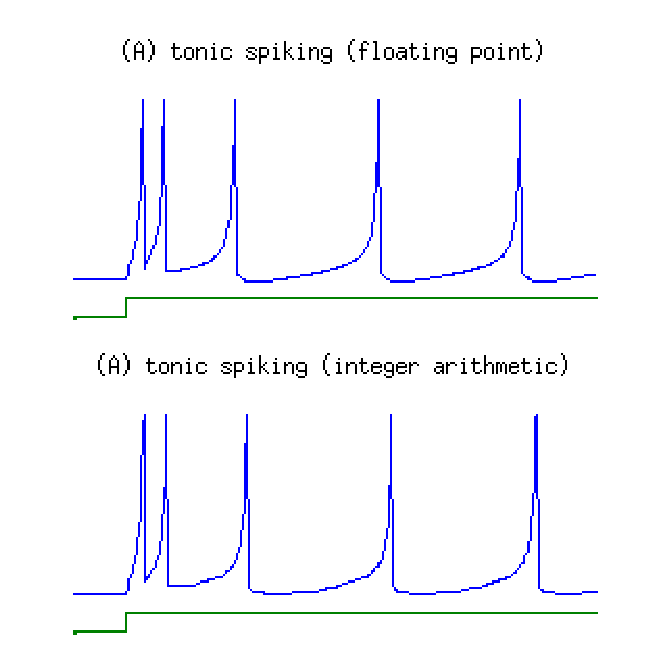
\includegraphics[scale=0.6]{imgs/izh_tonic}
\caption{Tonic spiking of a neuron.\label{fig:tonic}}
\end{figure}

\begin{figure}
\centering
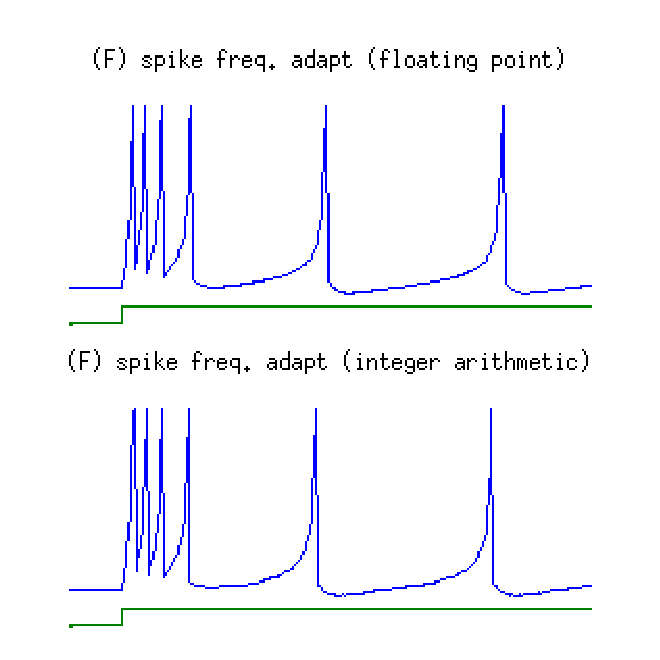
\includegraphics[scale=0.6]{imgs/izh_spike_freq_adapt}
\caption{Spike frequency adaptation of a neuron.\label{fig:freq}}
\end{figure}

\begin{figure}
\centering
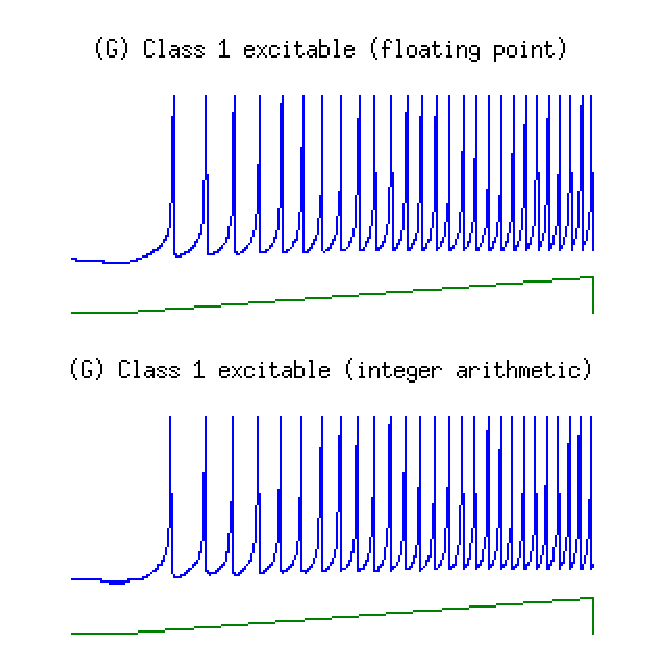
\includegraphics[scale=0.6]{imgs/izh_class_1_excitable}
\caption{Class 1 excitable neuron.\label{fig:excit1}}
\end{figure}


\subsection{Parallel Design}
The algorithm written on the multi-core parallel SpiNNaker system is a translation of sequential MATLAB code used in \cite{Polychron:Izhi}.
Instead of dealing with lists of neurons, we were able to simple use a variable per each neuron core.
Likewise, instead of using a two-dimensional array, where one dimension was the index of a neuron, 
we were able to simply use a one-dimensional array per each neuron core.
Arguably, the parallel implementation on the SpiNNaker was easier to design due to the code only ever acting locally on one core.

We used the weight modification rule proposed by Levy to categorize an input set of letters \cite{SynGen:Levy, SynGen2:Levy}.

We implemented a single-layer perception as a proof of concept to demonstrate synaptogenesis on the SpiNNaker board. In our network, every input node broadcasts a data packet to six of the output nodes. To simulate the creation and rewiring of synapses, not all messages are registered by the output neurons. 

Each packet received by an output node is looked up in the output node's local list of incoming connections. If the address from the packet is not listed in the incoming connections list, it will be ignored, and no further computation will be done.

Synaptic connectivity is broken when weights fall below some negative threshold. More specifically, when an average running weight dropped below \(-\delta\) for some \(\delta > 0\), the link is considered disconnected.

New connections are established between nodes when an average rate of activity drops below 25\%. In this case, the next data packet received from a muted neuron becomes unmuted, in hopes to raise the average rate of activity.

We combined the typical STDP mechanisms \cite{FBSTDP:Davies} with synaptogenetic formulas from \cite{SynGen:Levy, SynGen2:Levy} to created a new synaptic plasticity mechanism, which we refer to as synaptogenetic spike time dependent plasticity (SSTDP). This mechanism, implemented locally on each postsynaptic neuron, handles both synaptic weight and network-level topological modifications.

\section{Outcomes}
\IEEEPARstart{A}fter training the network on 1000 letters pixel-by-pixel, we were able to
observe the oscillatory property described by Izhikevich \cite{Polychron:Izhi}.
The output neurons initially fire at a frequency of $0.476 Hz$, which increases gradually.
This agrees with our hypothesis that polygroup behavior is possible on a spiking neural network architecture.
Refer to Figure~\ref{fig:spikes} for a plot of the output spike times.

\subsection{Results}

\begin{figure}
\centering
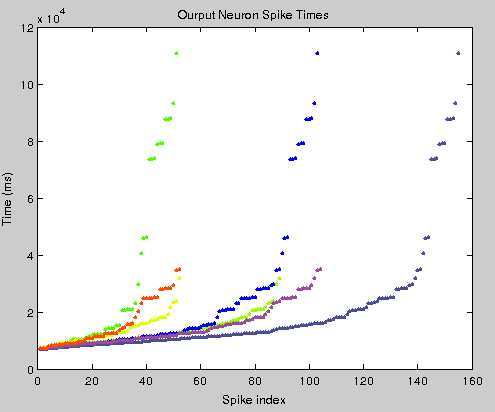
\includegraphics[scale=0.4]{imgs/spikes}
\caption{The spike times of output neurons are shown in the diagram above. 
Each neuron is represented by a different shade of color.
Some neurons share the same spiking patterns, so there are not 16 distinct curves.
The curves represent the timings when each neuron fires.\label{fig:spikes}}
\end{figure}

The SpiNNaker machine used for our experiment was powered solely by USB. 
The total power consumption of the simulation was at most 4 Watts, 
which is less than $75\%$ of the corresponding simulation on a ThinkPad T530 Laptop.

Spikes were delivered from the host machine to the SpiNNaker board in serial. 
Due to the clocking differences between the host machine and SpiNNaker board, 
we slowed down the simulation by a factor of 1000. 
Moreover, the internal SpiNNaker messages are prone to packet loss. 
Regardless of these shortcomings, the SpiNNaker simulation produced expected results.


% TODO: Nishant
\subsection{Conclusion}
Through empirical evidence, we have shown that by taking advantage of a spiking neural network architecture such as the SpiNNaker, 
we can implement a high performance energy efficient neural network system. 
Without the computation drawbacks of back-propagation, or the growing space complexity of global variables, 
we are able to train a network on a machine that uses less than 5 Watts of energy \cite{ArchOverV:Furber}.
% http://neuromorphs.net/nm/raw-attachment/wiki/2013/uns13/Power_analysis_of_large_scale_real_time_neural_networks_on_SpiNNaker.pdf
Furthermore, we have demonstrated that a neural network can produce outstanding results by having its input be fed in series as opposed to in parallel.


% Step by step nn

\section{Pitfalls}
\IEEEPARstart{S}{ome} disadvantages are present when considering our approach 
for synaptogenesis on the SpiNNaker. 
Programming parallel applications is a challenge in its own right, 
but a lack of floating point support on the 
SpiNNaker system \cite{ArchOverV:Furber} compounds the difficulty, 
especially when the neural dynamics parameters and coefficients in the differential equations 
of Izhikevich's simple neural model are floating point numbers \cite{Spikes:Izhi}. 
To get around this, we rationalized all coefficients in the equations and multiplied the 
entire set of equations by the lowest common multiple of the denominators of 
the rationalized coefficients. 
This incurred a slight loss of precision, but not so much that the models we 
used exhibited different neural activity behavior than their original counterparts 
with the same input. 
Source code illustrating this is available upon request.

Also, due to inherent limitations to Ethernet speed, our simulation had to be slowed by a factor of 1000 to allow for reliable I/O communications with the host machine. There are plans in motion to accommodate for faster communication between SpiNNaker boards and host machines, so this will no longer be an issue once higher speed I/O is achieved.

% TODO: Nishant
\section{Further Study}
\IEEEPARstart{T}{his} paper reveals multiple questions that still need to be examined further. 
A key feature of the SpiNNaker machine is its ability to connect to other SpiNNaker chips for scalable performance.
Future papers can examine the performance of a network of multiple SpiNNaker chips together.
It's been shown that with ``quarter of a million neurons, 
tens of millions of synapses and dynamic activity of over a billion synaptic events per second can be delivered within a 30 W power envelope. \cite{power:Strom}''



% if have a single appendix:
%\appendix[Proof of the Zonklar Equations]
% or
%\appendix  % for no appendix heading
% do not use \section anymore after \appendix, only \section*
% is possibly needed

% use appendices with more than one appendix
% then use \section to start each appendix
% you must declare a \section before using any
% \subsection or using \label (\appendices by itself
% starts a section numbered zero.)
%


\appendices
\section{Shannon's Entropy and Mutual Information}
Entropy is the measure of information in a system. 
We use it to measure the unpredictability of information content.
Mutual information is a measure of the mutual dependence between two random variables.
It can be expressed in terms of entropy.

\subsection{Entropy}
The entropy of a series of data is the expected value of the information.

\vspace{0.2cm}
\begin{math}
H(X) = E[I(X)]
\end{math}
\vspace{0.2cm}

Information has the units of bits when the logarithm in the equation below is in base 2.

\vspace{0.2cm}
\begin{math}
I(X) = -log(P(X))
\end{math}
\vspace{0.2cm}


\subsection{Mutual Information}
The mutual information between two random variables $X$ and $Y$ is expressed in the equation below.

\vspace{0.2cm}
\begin{math}
I(X;Y) = \sum_{y \in Y} \sum_{x \in X} p(x, y) log( \frac{p(x,y)}{p(x) p(y)})
\end{math}
\vspace{0.2cm}

An equivalent, but simpler equation is in terms of only entropy of the $X$ and $Y$ random variables.

\vspace{0.2cm}
\begin{math}
I(X;Y) = H(X) - H(X|Y)
\end{math}
\vspace{0.2cm}

\section{Floating point vs. Integer arithmetic}
Figures~\ref{fig:tonic} through~\ref{fig:excit1} and~\ref{fig:excit2} through~\ref{fig:accomod8} illustrate the comparison between using the floating point arithmetic found in Izhikevich's original neural models \cite{Spikes:Izhi} and the integer arithmetic we formulated for our experiment. In most cases the behavior of each is indistinguishable from one another. However, note the visually apparent rounding errors figures~\ref{fig:excit2} and~\ref{fig:reson8r}. Since our experiment used exclusively the tonic spiking integer arithmetic (with slight modifications to distinguish between excitatory and inhibitory neurons) from figure~\ref{fig:tonic}, the rounding errors were not a problem.

\begin{figure}
\centering
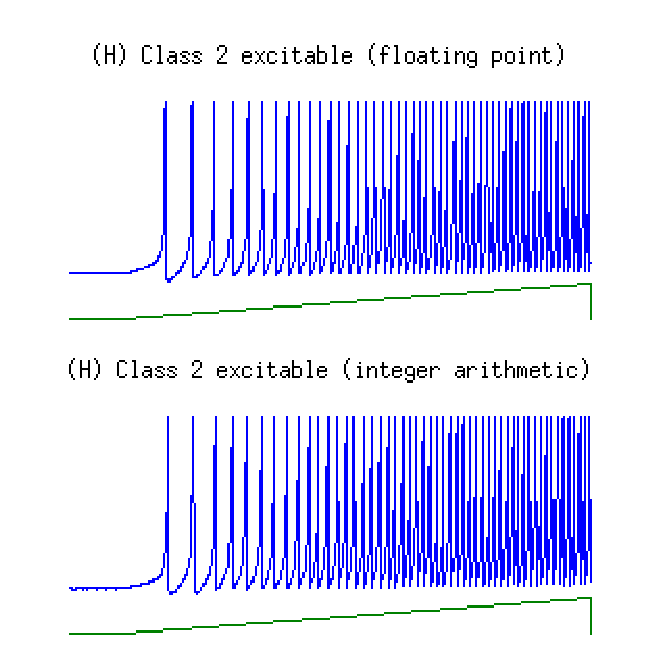
\includegraphics[scale=0.6]{imgs/izh_class_2_excitable}
\caption{Class 2 excitable neuron.\label{fig:excit2}}
\end{figure}

\begin{figure}
\centering
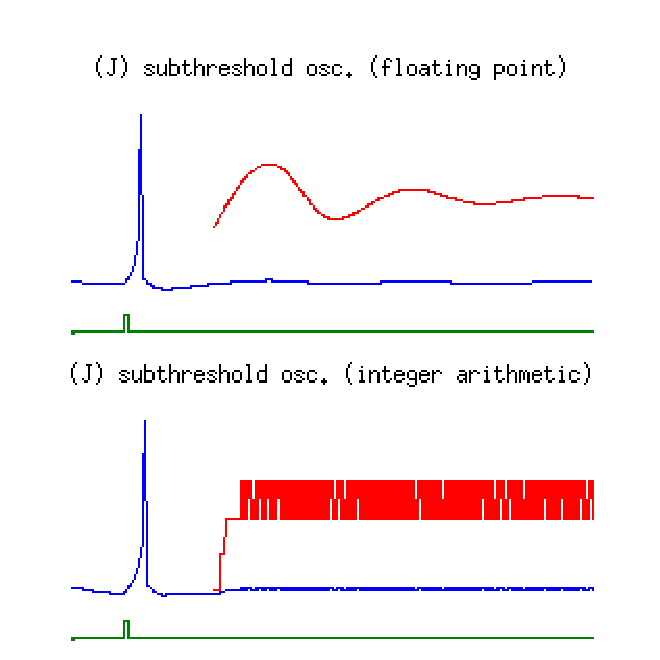
\includegraphics[scale=0.6]{imgs/izh_subthreshold_osc}
\caption{Subthreshold oscillatory neuron.\label{fig:osc}}
\end{figure}

\begin{figure}
\centering
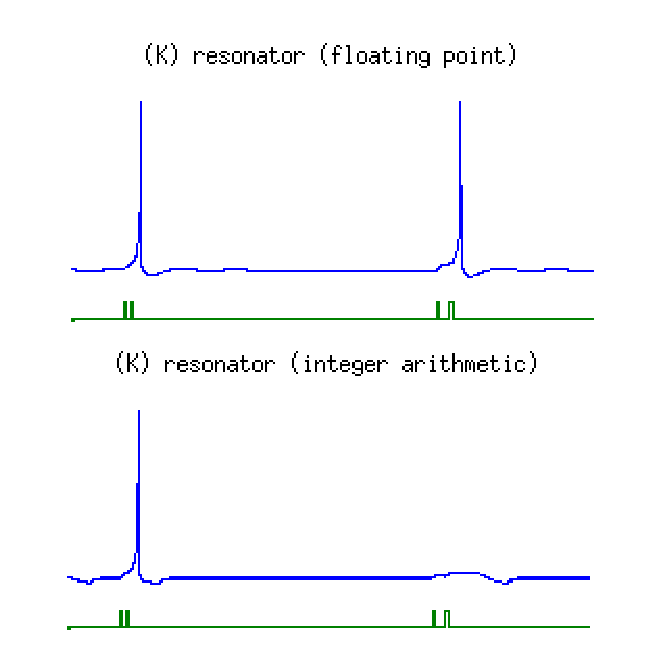
\includegraphics[scale=0.6]{imgs/izh_resonator}
\caption{Spiking resonator neuron.\label{fig:reson8r}}
\end{figure}

\begin{figure}
\centering
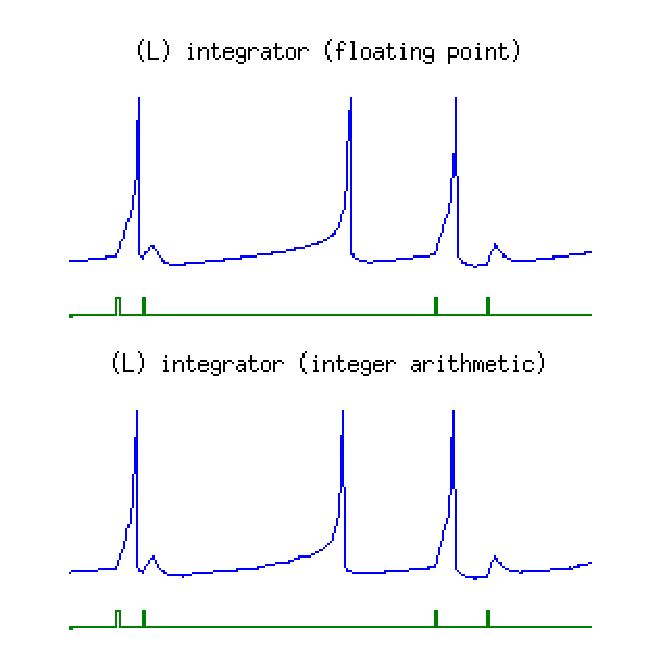
\includegraphics[scale=0.6]{imgs/izh_integrator}
\caption{Integrator neuron.\label{fig:integr8r}}
\end{figure}

\begin{figure}
\centering
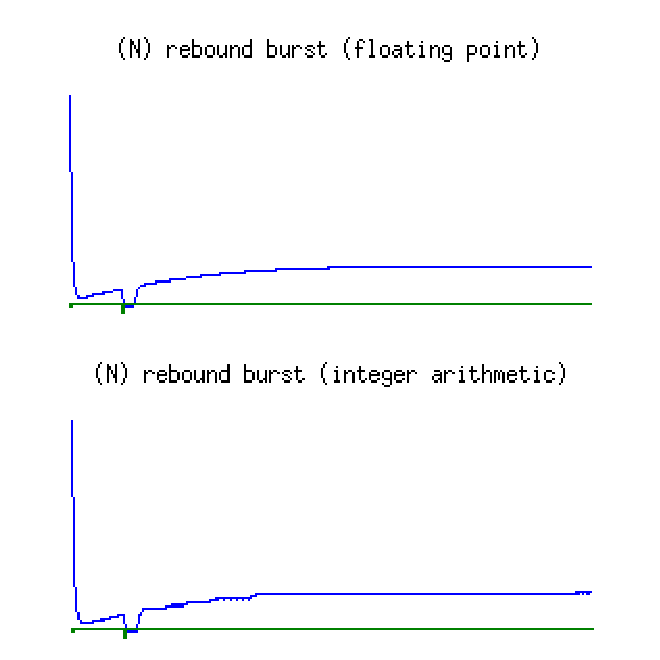
\includegraphics[scale=0.6]{imgs/izh_rebound_burst}
\caption{Rebound burst neuron.\label{fig:rebound}}
\end{figure}

\begin{figure}
\centering
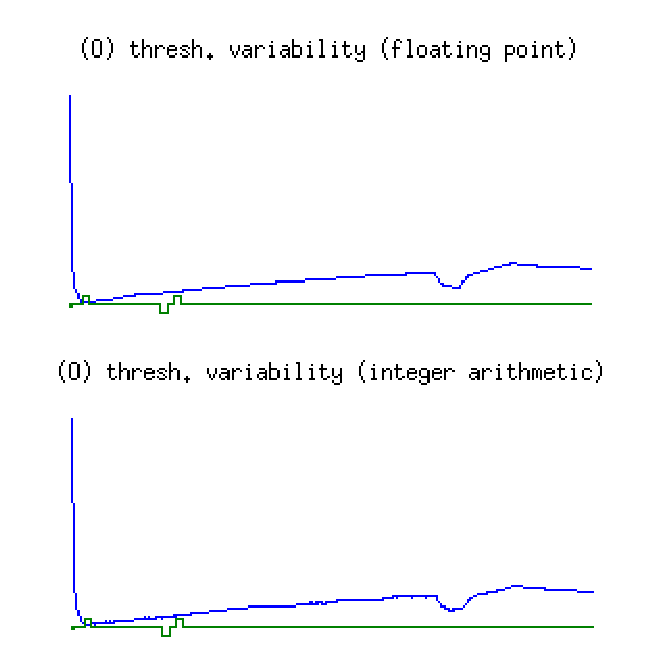
\includegraphics[scale=0.6]{imgs/izh_thresh_variability}
\caption{Threshold variability neuron.\label{fig:threshvar}}
\end{figure}

\begin{figure}
\centering
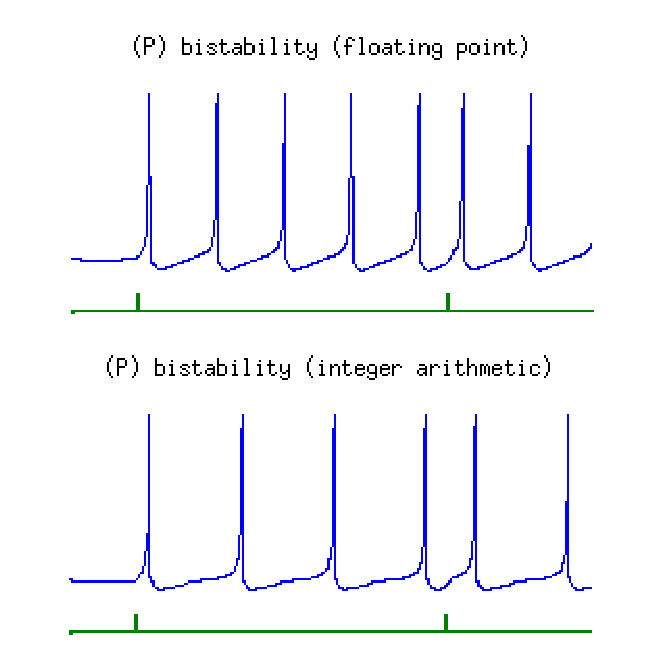
\includegraphics[scale=0.6]{imgs/izh_bistability}
\caption{Bistability neuron.\label{fig:bistable}}
\end{figure}

\begin{figure}
\centering
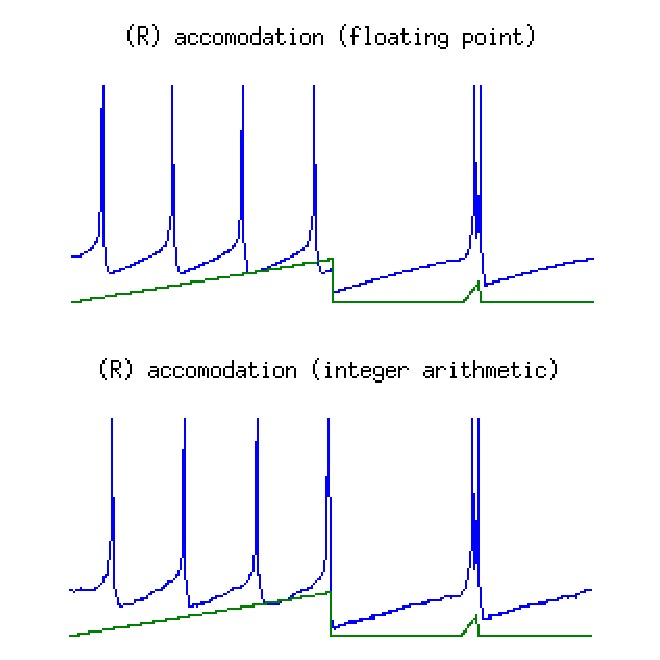
\includegraphics[scale=0.6]{imgs/izh_accomodation}
\caption{Accommodation neuron.\label{fig:accomod8}}
\end{figure}


\newpage

% use section* for acknowledgement
\section*{Acknowledgment}


The authors would like to thank Professor Worthy Martin, Associate Professor of Computer Science at the University of Virginia. The authors also greatly appreciate the generosity of the SpiNNaker team from the APT Research Group at the University of Manchester, who were gracious enough to not only loan the neuro-computing device, but also to help us debug issues whenever possible.


% Can use something like this to put references on a page
% by themselves when using endfloat and the captionsoff option.
\ifCLASSOPTIONcaptionsoff
  \newpage
\fi



% trigger a \newpage just before the given reference
% number - used to balance the columns on the last page
% adjust value as needed - may need to be readjusted if
% the document is modified later
%\IEEEtriggeratref{8}
% The "triggered" command can be changed if desired:
%\IEEEtriggercmd{\enlargethispage{-5in}}

% references section

% can use a bibliography generated by BibTeX as a .bbl file
% BibTeX documentation can be easily obtained at:
% http://www.ctan.org/tex-archive/biblio/bibtex/contrib/doc/
% The IEEEtran BibTeX style support page is at:
% http://www.michaelshell.org/tex/ieeetran/bibtex/
%\bibliographystyle{IEEEtran}
% argument is your BibTeX string definitions and bibliography database(s)
%\bibliography{IEEEabrv,../bib/paper}
%
% <OR> manually copy in the resultant .bbl file
% set second argument of \begin to the number of references
% (used to reserve space for the reference number labels box)


\begin{thebibliography}{23}

\bibitem{CorrMatr:Levy}
D.~Adelsberger-Mangan and W.~Levy in \emph{International Joint Conference on Neural Networks 4}, 1992

\bibitem{StatDepRed:Levy}
D.~Adelsberger-Mangan and W.~Levy in \emph{Biological Cybernetics 67}, 1992, pp. 469-477

\bibitem{SynGen:Levy}
D.~Adelsberger-Mangan and W.~Levy in \emph{Biological Cybernetics 70}, 1993, pp. 81-87

\bibitem{backprop:Qun}
Q.~Dai and N.~Liu in \emph{Neurocomputing Vol. 94}, 2012, pp.152-158

\bibitem{FBBPSTDP:Davies}
S.~Davies et al. in \emph{Proceedings of International Joint Conference on Neural Networks}, San Jose, CA, 2011

\bibitem{FBSTDP:Davies}
S.~Davies et al. in \emph{Neural Networks 32} 2012, pp. 3–14

\bibitem{RTS:Davies}
S.~Davies et al. in \emph{Proceedings of the 8th ACM International Conference on Computing Frontiers}, New York, NY, 2011, Article No. 15 

\bibitem{ArchOverV:Furber}
S.~Furber et al. in \emph{IEEE Transactions on Computers, Vol. 62, No. 12}, 2013, pp. 2454-2467

\bibitem{BioMPA:Furber}
S.~Furber and A.~Brown in \emph{Ninth International Conference on Application of Concurrency to System Design}, 2009, pp. 3-12

\bibitem{NSE:Furber}
S.~Furber and S.~Temple in \emph{Journal of the Royal Society Interface 4}, 2007, pp. 193-206

\bibitem{HierarchMPA:Galluppi}
F.~Galluppi et al. in \emph{Proceedings of the 9th conference on Computing Frontiers}, New York, NY, 2012, pp. 183-192

\bibitem{RankPolychron:Galluppi}
F.~Galluppi and S.~Furber in \emph{Internation Joint Conference on Neural Networks}, San Jose, CA, 2011, pp. 943-950 

\bibitem{STDPonset:Humble}
J.~Humble et al. in \emph{From Brains to Systems}, Springer New York, 2011, pp. 19-31

\bibitem{Spikes:Izhi}
E.~Izhikevich in \emph{IEEE Transactions on Neural Networks 14}, 2003, pp. 1569-1572

\bibitem{Polychron:Izhi}
E.~Izhikevich in \emph{Neural Computation 18}, 2006, pp. 245-282

\bibitem{deSNN:Kasabov}
N.~Kasabov et al. in \emph{Neural Networks 41}, 2013, pp. 188-201

\bibitem{SynGen2:Levy}
W.~Levy in \emph{Neurocomputing 58-60}, 2004, pp. 343-350

\bibitem{Interconnection:Navaridas}
J.~Navaridas et al. in \emph{Proceedings of the 23rd international conference on Supercomputing}, 2009, pp. 286-295 

\bibitem{MPI:Plana}
L.~Plana et al. in \emph{IEEE Design and Test archive, Vol. 24 No. 5}, 2007, pp. 454-463

\bibitem{GALS:Plana}
L.~Plana et al. in \emph{ACM Journal on Emerging Technologies in Computing Systems, Vol. 7, No. 4}, 2011

\bibitem{Fast:Rast}
A.~Rast et al. in \emph{Neural Networks 24}, 2011, pp. 961-978

\bibitem{DNN:Siniscalchi}
S.~Siniscalchi et al. in \emph{Neurocomputing Vol 106}, 2013, pp. 148-157

\bibitem{Efficient:Sharp}
T.~Sharp et al. in \emph{Journal of Neuroscience Methods 210}, 2012, pp. 110-118

\bibitem{ENNtAT:Stanley}
K.~Stanley and R.~Miikkulainen in \emph{Evolutionary Computation, Vol. 10 No. 2}, 2002, pp. 99-127

\bibitem{power:Strom}
E.~Stromatias et al. in \emph{The International Joint Conference on Neural Networks}, 2013, pp. 1-8

\bibitem{RO:Thorpe}
S.~Thorpe and J.~Gautrais in \emph{Computational Neuroscience; trends in research}, 1998, pp. 113-118

\bibitem{img:N}
Image, unedited, taken from http://ehumanbiofield.wikispaces.com/neurons+WG under the Creative Commons license (http://creativecommons.org/licenses/by-sa/3.0/)

\end{thebibliography}

\end{document}
